\chapter{EEG Mismatch negativity data\label{Chap:data:mmn}}

This chapter describes the analysis of a 128-channel single subject EEG data set acquired from a study of mismatch negativity in the auditory system \cite{marta_mmndcm}. We thank Marta Garrido for providing us with these data. The experiment comprised an auditory oddball paradigm in which subjects heard standard (500Hz) and deviant (550Hz) tones, occuring 80\% (480 trials) and 20\% (120 trials) of the time, respectively, in a pseudo-random sequence subject to the constraint that two deviant tones did not occur together.

EEG data were recorded with a Biosemi\footnote{BioSemi: \url{http://www.biosemi.com/}} system at 128 scalp electrodes and a sampling rate of 512Hz. Vertical and horizontal eye movements were monitored using EOG electrodes. See \cite{marta_mmndcm} for full details of experimental stimuli and recording. To proceed with the data analysis, first download the  data set from the SPM website\footnote{EEG MMN dataset: \url{http://www.fil.ion.ucl.ac.uk/spm/data/eeg\_mmn/}}. The data comprises a file called \texttt{subject1.bdf} whose size is roughly 200MB. We will refer to the directory in which you have placed it as \texttt{DATA\_DIR}. This chapter takes you through different stages of analysis:

\begin{itemize}
\item{Preprocessing}
\item{Sensor space analysis}
\item{Source reconstruction}
\item{Dynamic Causal Modelling}
\end{itemize}

\section{Preprocessing}

Unlike preprocessing in SPM8 which consisted of a sequence of steps applied to a dataset using the GUI, preprocessing in SPM12 is most conveniently done by building and configuring a batch pipeline and then running it. The advantage of that is that a batch pipeline can immediately be applied to another dataset with perhaps minor adjustments. It is also possible to call preprocessing functions from a more low-level scripts. These scripts can be generated from the history SPM saved in preprocessed datasets and then modified.  There is also an example \matlab\ script under \texttt{man$\backslash$example\_scripts$\backslash$history\_subject1.m} in the SPM distribution which repeats the preprocessing route we take here.

\subsection{Simple conversion and reviewing}

At the \matlab\ prompt type \texttt{spm eeg}, from the \textsc{Convert} dropdown menu  select \textsc{Convert}. At the prompt ``Define settings?'' select ``just read'',  select the \texttt{subject1.bdf} file and press "Done". SPM will now read the original Biosemi format file and create an SPM compatible data file, called \texttt{spmeeg\_subject1.mat} and \texttt{spmeeg\_subject1.dat} in the directory containing the original data file (\texttt{DATA\_DIR}). From "Display" dropdown meny select "M\EEG". In the file selection dialogue that comes up select \texttt{spmeeg\_subject1.mat} and press "Done". The file will now be opened in the SPM reviewing tool. By default the tool will be opened on the 'history' tab that shows the sequence of preprocessing steps applied to the dataset until now (in this case there is just single line for 'Conversion'). You can switch to 'channels' and 'trials' tabs to see the list of channels and events in  the dataset. Then switch to 'EEG' tab to review the continuous data. Note that due to large DC shifts in this particular datasets all the channels initially look flat and it is necessary to zoom in to actually see the EEG traces. 

\subsection{Preparing batch inputs}
Press the 'Prepare SPM file' button in the top right corner of the reviewing tool window. A menu will appear in the SPM interactive window (the small window usually located at the bottom left). Similar functionality can also be accessed without the reviewing tool by choosing \textsc{Prepare} from the \textsc{Convert} dropdown menu. Here we will prepare in advance some inputs that will be necessary for the subsequent preprocessing stages. The reason this needs to be done is that all inputs to the batch tool must be provided in advance before hitting the 'Run' button. Therefore, for some steps where specifying inputs interactively using information stored in the dataset is much simpler interactive GUI tools are provided in the 'Prepare' menu. As the first step we will make a list of channels to be read. The original files contains some unused channels that do not need to be converted and we can exclude them from the beginning. From 'Batch inputs' menu select 'Channel selection'. A popup window will appear with the list of all channels in the dataset. A subset of channels can be selected (use Shift- and Ctrl- clicks if necessary to select multiple items). Select all EEG channels from A1 to D32. In addition select 3 channels that were used in the experiment to record EOG: EXG1, EXG2 and EXG3. Press 'OK' and save the selection as a mat file named e.g 'channelselection.mat'.

Next we will prepate an input for the Montage step. This step will derive vertical and horizontal EOG channels buy subtracting pairs of channels located above and below the eye and below and lateral to the eye respectively. The way to create the montage solely using GUI for this particular datasets requires several steps. First we will change the channel type of the channels containing EOG. Select  'EOG' from 'Channel types' menu and in the channel list thatl comes up select EXG1, EXG2 and EXG3 channels and press OK. Next  from 'Batch inputs' menu select 'Montage' and there select 'Re-reference'. In the channel list that comes up press 'Select all channels', press OK and save the montage e.g. as 'avref.mat'. This montage subtracts the average of all channels from each channels which is called 'conversion to average reference'. We would now like to add to the montage two extra lines deriving the EOG channels. To do that from the same 'Montage' submenu select 'Custom montage' and in the window that appears press 'Load file' and load the previously saved 'avref.mat'.  Click on the button at the top left of the montage table to select the whole table and press Ctrl-C (or equivalent on your system). Now press 'OK' , open 'Custom montage' tool again press the top left button again and press Ctrl-V (or equivalent). On some systems it instead of pressing Ctrl-C and Ctrl-V it is better to select 'Copy' and 'Paste' respectively after right-clicking the corner button.   Now scroll to the bottom of the table. On line 129 write 'HEOG' instead of 'EXG1'. On line 130 write 'VEOG' instead of 'EXG2'. Click to select the whole of line 131 and press 'Delete' (or equivalent). Finally scroll to the bottom right of the table and  add '-1' in line 129 in the column for 'EXG2' and in line 130 in the column for 'EXG3'. This defines the HEOG channel as the difference of EXG1 and EXG2 and VEOG as the difference of EXG2 and EXG3. Save the montage by  pressing the 'Save as' button and naming the file 'avref_eog.mat'. Press 'OK' to close the 'Custom montage' tool. 

Alternatively, it might be easier to create the montage using a short script available at  \texttt{example\_scripts} folder: \texttt{montage\_subject1.m}. Copy this script into \texttt{DATA\_DIR} and run it. This will generate a file named \texttt{MONT\_EXP.mat}}.

The final input we should prepare in advance is trial definition for epoching. Select 'Trial definition' from 'Batch inputs' menu.  Choose the peri-stimulus time window as \texttt{-100 400}. Choose 2 conditions. You can call the first condition ``standard''. A GUI pops up which gives you a complete list of all events in the EEG file. The standard condition had 480 trials, so select the type with value 1 and press OK. Leave 'Shift trials' at default 0. The second condition can be called ``rare''. The rare stimulus was given 120 times and has value 3 in the list. Select this trial type and press OK.  Leave 'Shift trials' at default 0.  Answer``no'' to the question  ``review individual trials'', and  save the trial definition as 'trialdef.mat'.The 'Run' button is now enabled. Press on it to run the batch and convert the dataset.

\subsection{Preprocessing step by step}

We will now build a complete batch pipeline for preprocessing and statistical analysis of the MMN dataset. We will start with running different steps one-by-one and then show how to chain these steps to run them all together. 

\subsubsection{Convert}
Select \textsc{Convert} from the \textsc{Convert} dropdown menu and this time answer 'yes' to 'Define settings?'. Conversion batch tool will appear. If you are not familiar with SPM batch, the tool presents the configuration structure as a tree where you can enter values and select different options from a list. For many options there are default settings. Options where user input must be provided are marked by '<-X' sign on the right of the window. All these entries must be specified to enable the 'Run' button (green triangle at the toolbar) and run the batch. In our case we will provide the raw dataset name and channel selection. Double-click on the row with 'File name' and select \texttt{subject1.bdf} file. Click on 'Channel selection' and in the list of option appearing below the configuration tree display click on 'Delete: All(1)'. This will remove the default setting of selecting all channels. Then click on 'New: Channel file'. An entry for 'Channel file' will appear under 'Channel selection'. Double-click on it and select the previously saved 'channelselection.mat' file. 

\subsubsection{Montage}
Select \textsc{Montage} from the \textsc{Preprocessing} dropdown menu. Montage batch tool will appear. Double-click on 'File name' and select the \texttt{spmeeg\_subject1.mat} file created by conversion. Click on 'Montage file name' and select the  'avref_eog.mat' (or \texttt{MONT\_EXP.mat}) file generated as described above. Run the batch. The progress bar appears and SPM will generate two new files \texttt{Mspmeeg\_subject1.mat} and \texttt{Mspmeeg\_subject1.dat}.

\subsubsection{Prepare}
The previous step also assigned default locations to the sensors, as this information is not contained in the original Biosemi \texttt{*.bdf} file. It is usually the responsibility of the user to link the data to sensors which are located in a coordinate system. In our experience this is a critical step. Here we will perform this step using 'Prepare' batch. Select \textsc{Prepare (batch)} from the \textsc{Convert} dropdown menu. Select \texttt{Mspmeeg\_subject1.mat} dataset as input. Click on 'Select task(s)' and from the options list select 'New: Load EEG sensors'. Under 'Select EEG sensors file' select 'sensors.pol' file provided with the example dataset and run the batch. At this step no new files will be generated but the same dataset will be updated.

\subsubsection{High-pass filter}
Filtering the data in time removes unwanted frequency bands from the data. Usually, for evoked response analysis, the low frequencies are kept, while the high frequencies are assumed to carry noise. Here, we will use a highpass filter to remove ultra-low frequencies close to DC, and a lowpass filter to remove high frequencies. We filter prior to downsampling because otherwise high-amplitude baseline shifts present in the data will generate filtering artefacts at the edges of the file. Select \textsc{Filter} from the \textsc{Preprocessing} dropdown menu. Select \texttt{Mspmeeg\_subject1.mat} dataset as input.  Click on 'Band' and choose 'Highpass'. Double-click on 'Cutoff(s)' and enter 0.1 as the cutoff frequency. Run the batch. The progress bar will appear and the resulting filtered data will be saved in files \texttt{fMspmeeg\_subject1.mat} and \texttt{fMspmeeg\_subject1.dat}. 

\subsubsection{Downsample}
Here, we will downsample the data in time. This is useful when the data were acquired like ours with a high sampling rate of 512 Hz. This is an unnecessarily high sampling rate for a simple evoked response analysis, and we will now decrease the sampling rate to 200 Hz, thereby reducing the file size by more than half.  Select \textsc{Downsample} from the  \textsc{Preprocessing} dropdown menu and select the \texttt{fMspmeeg\_subject1.mat} file. Choose a new sampling rate of 200 (Hz). The progress bar will appear and the resulting data will be saved to files \texttt{dfMspmeeg\_subject1.mat} and \texttt{dfMspmeeg\_subject1.dat}.

\subsubsection{Low-pass filter}
 Select \textsc{Filter} from the \textsc{Preprocessing} dropdown menu. Select \texttt{dfMspmeeg\_subject1.mat} dataset as input.  Keep the band at default  'Lowpass'. Double-click on 'Cutoff(s)' and enter 30 as the cutoff frequency. Run the batch. The progress bar will appear and the resulting filtered data will be saved in files \texttt{fdfMspmeeg\_subject1.mat} and \texttt{fdfMspmeeg\_subject1.dat}. 

\subsubsection{Epoch}
Here we will epoch the data using the previously created trial definition file. Note that it is possible to create trial definition one one file and use it on a different file as long as events are coded the same way in both files.  Select \textsc{Epoch} from the \textsc{Preprocessing} dropdown menu. Select the \texttt{fdfMspmeeg\_subject1.mat} file as input. For 'How to define trials' select 'Trial definition file' and choose the previously saved 'trialdef.mat'. The progress bar will appear and the epoched data will be saved to files \texttt{efdfMspmeeg\_subject1.mat} and \texttt{efdfMspmeeg\_subject1.dat}. 

\begin{figure}
\begin{center}
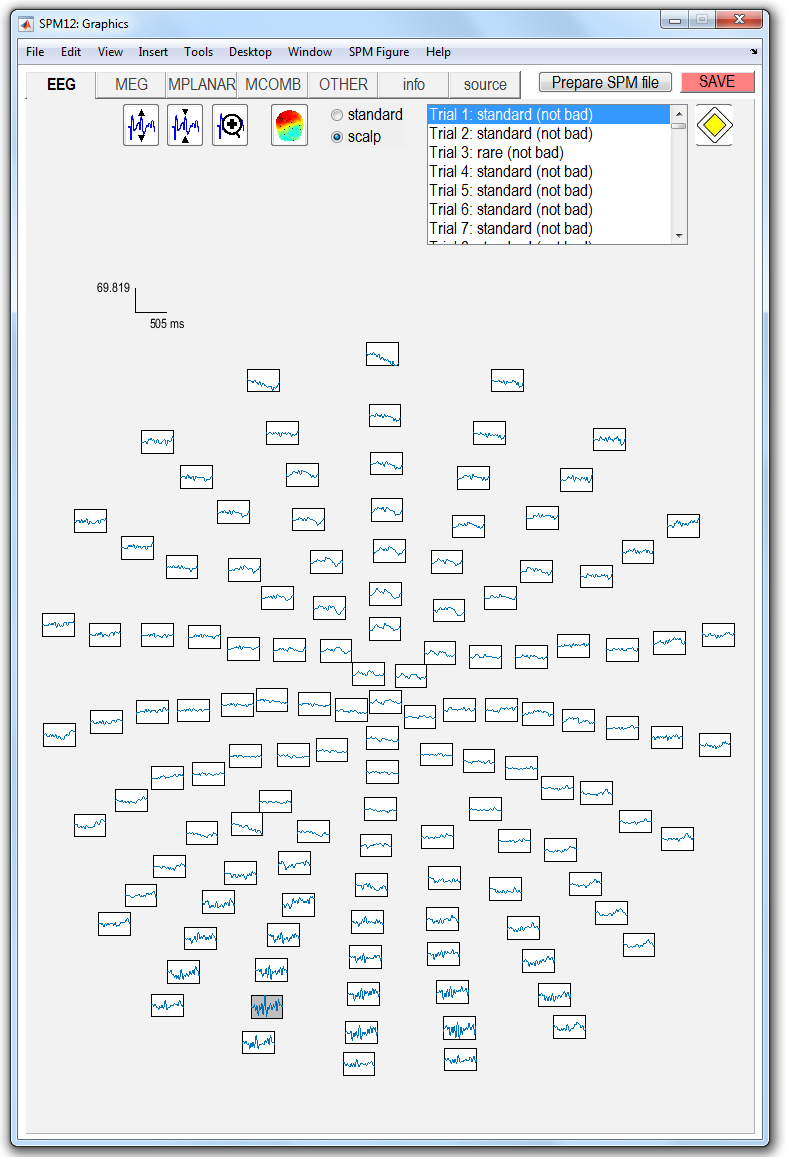
\includegraphics[width=150mm]{mmn/topo1}
\caption{\em Scalp topography of single trial MMN EEG data. Channel 14, second-row from bottom, left hemisphere contains (slightly) higher variability data than the others. This channel is to be marked as artefactual (ie. 'bad').
\label{topo1}}
\end{center}
\end{figure}

\subsubsection{Artefacts}
 A number of different methods of artefact removal are implemented in SPM. Here, we will demonstrate a simple thresholding method. However, before doing so, we will look at the data in the display:
\begin{itemize}
\item{Choose ``M/EEG'' from the ``Display'' dropdown menu.}
\item{Select the \texttt{efdfMspmeeg\_subject1.mat} file.}
\item{Click on the ``EEG'' tab.}
\item{Press the ``scalp'' radio button.}
\end{itemize}
The time-series for the first trial will then appear in the topographical layout shown in Figure~\ref{topo1}.

You will see that Channel 14, second-row from bottom, left hemisphere, contains (slightly) higher variability data than the others .
Right-click on the channel; this tells you that this channel is ``A14''. You will also see as an entry in this menu ``bad: 0''. Select this entry, and click the left button. This will make the menu disappear, but the channel now has a grey background. You have marked this channel as bad. Click on ``save''in the top-right corner. This channel will then be ignored in subsequent processing. In fact this channel probably doesn't need removing, but we do so for teaching purposes only.
\\
\\
Select \textsc{Detect artefacts} from the \textsc{Preprocessing} dropdown menu. Select the \texttt{efdfMspmeeg\_subject1.mat} file as input.  Double click ``How to look for artefacts'' and a new branch will appear. It is possible to define several sets of channels to scan and several different methods for artefact detection. We will use simple thresholding applied to all channels. Click on ``Detection algorithm'' and select ``Threshold channels'' in the small window below. Double click on ``Threshold'' and enter 80 (in this case $\mu V$). The batch is now fully configured. Run it by pressing the green button at the top of the batch window. 

This will detect trials in which the signal recorded at any of the channels exceeds 80 microvolts (relative to pre-stimulus baseline). These trials will be marked as artefacts. Most of these artefacts occur on the VEOG channel, and reflect blinks during the critical time window. The procedure will also detect channels in which there are a large number of artefacts (which may reflect problems specific to those electrodes, allowing them to be removed from subsequent analyses).

In this case, the Matlab window will show:
\begin{verbatim}
1 bad channels: A14 
82 rejected trials: 3    4    5    7   26   27   28    [...]
Done    'M/EEG Artefact detection'
Done
\end{verbatim}
A new file will also be created, \texttt{aefdfMspmeeg\_subject1.mat}.

There are also interactive artefact removal routines available from \texttt{Toolbox} $\rightarrow$ \texttt{MEEG tools} $\rightarrow$  \texttt{Fieldtrip visual artifact rejection}.

\subsubsection{Averaging}
To produce an ERP click on \textsc{Averaging} and select the \texttt{aefdfMspmeeg\_subject1.mat} file. At this point you can perform either ordinary averaging or ``robust averaging''. Robust averaging makes it possible to supress artefacts automatically without rejecting trials or channels completely, but just the contaminated parts. For robust averaging select 'Robust' under 'Averaging type'.  Also select ``yes'' for ``Compute weights by condition'' \footnote{In this case we do not want to pool both conditions together because the number of standard and rare trials are quite different.} and press ``Enter'' to accept the default ``Offset of the weighting function''. A new dataset will be generated \texttt{maefdfMspmeeg\_subject1.mat}. 

Open the averaged dataset in the reviewing tool. To look at the ERP, click on the EEG tab, and press the ``scalp'' radio button. Now hold  the Shift button down on the keyboard whilst selecting trial 2 with the left mouse button in the upper right corner of the graphics window. This will overlay responses to standard and rare trials on the same figure axes.

Now press the ``plus'' icon at the top of this graphics window and select channel C23 (seventh central channel down from the top) with a left mouse click. This will plot the ERPs shown in Figure~\ref{c23}. This completes the preprocessing step.
\begin{figure}
\begin{center}
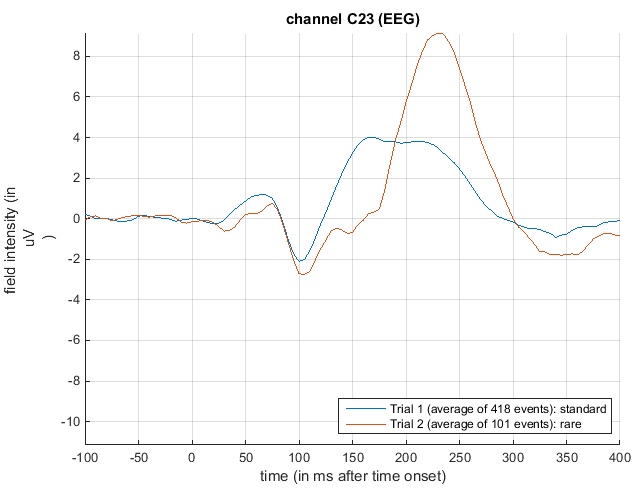
\includegraphics[width=120mm]{mmn/erp_c23}
\caption{\em ERPs at channel C23 (CZ) for standard and rare tones. The ERP curve for rare tones lies underneath that for standard tones between 100 and 180ms. This corresponds to the mismatch negativity signal in this subject. \label{c23}}
\end{center}
\end{figure}

\subsection{Automatisation of preprocessing}
The preprocessing steps we performed separately for instructive puproses can all be run sequentially as part of a pipeline. It is also useful in many cases to be able to easily change the input raw file and run the same pipeline on a different input dataset from a different session or subject. There are two ways to build a pipeline in SPM. One way is to use the batch tool as we did above but instead of configuring and running each step separately to configure all the steps as a chain and run them together. The second way is to use a script calling the low-level preprocessing functions. Such a script can be generated semi-automatically from the history of a pre-processed file. For more complicated pipelines there can be scripts that configure and run batch pipelines for some steps with some processing with the user's own code in between. In different parts of SPM the 'division of labour' between the code that is part of the batch tools and more low-level code can be different. So for M/EEG preprocessing running low-level functions without the batch is quite simple whereas for statistics or source reconstruction it is much easier to use the batch code. Some examples will be provided below. 

\subsubsection{Building a batch pipeline}
Press the 'Batch' button at the bottom right of the SPM menu window.  An empty batch tool will be open. Processing steps can now be added via the menu. From the SPM menu in the batch window select M/EEG submenu and in the submenu select 'Conversion'. The conversion configuration tree will appear. Configure it as described above (the 'Conversion' section).  Now without running the batch or closing the batch window go back to the M/EEG submenu and select the 'Preprocessing' sub-submenu and from there 'Montage'.  On the left of the batch window 'Montage' will appear in module list.  Click on it to switch to the montage configuration interface.  Now comes the critical difference from the previously described step-by-step processing. Single-click on 'File name'. 'Dependency' button will appear at the bottom left part of the batch window. Press this button. A list will appear with the outputs of all the previous batch modules. In our case there is only one item in the list - the output of conversion. Select it and press 'OK'. The rest of montage configuration is as described in the 'Montage' section above. Now continue with 'Prepare' and the other modules in similar fashion. Once batch is fully configured it can be run by pressing the green triangle button. 

Note that you can use 'Delete' batch tool from the 'Other' submenu to delete the intermediate datasets that you don't need once the final processing step has been completed. Finally, you can save the full batch pipeline as Matlab code. To do that select 'Save batch' from the 'File' menu of the batch tool. At the bottom of the dialogue box that appears, select 'Matlab .m script file'. Save the batch as e.g. 'mmnbatch.m'. You can then open the batch .m file either in the batch tool to reproduce the configured pipeline or in the Matlab editor. The generated Matlab code is quite straightforward to interpret. It basically creates a data structure closely corresponding to the structure of the configuration tree in the batch tool. The structure can be easily modified e.g. by replacing one input dataset name with another. Things one should be careful about is not changing the kind of brackets around different variables and also paying attention whether some list is a row or column cell array of strings which might be important. Once 'matlabbatch' structure is created by the code (or loaded from a .mat file) it can immediately be run from a script without the need to load it in a batch GUI. The command for that is \texttt{spm\_jobman('run', matlabbatch)}.

\subsubsection{Generating scripts from history}
The evoked response file (and every other SPM MEEG data file) contains a history-entry which stores all of the above preprocessing steps. You can take this history and produce a script that will re-run the same analysis which you entered using the GUI. See the ``history'' tab in the ``info'' section when displaying the data. Chapter \ref{Chap:eeg:preprocessing} provides more details on this.

\section{Sensor space analysis}

A useful feature of SPM is the ability to use Random Field Theory to correct for multiple statistical comparisons across N-dimensional spaces. For example, a 2D space representing the scalp data can be constructed by flattening the sensor locations and interpolating between them to create an image of MxM pixels (when M is user-specified, eg M=32). This would allow one to identify locations where, for example, the ERP amplitude in two conditions at a given timepoint differed reliably across subjects, having corrected for the multiple t-tests performed across pixels. That correction uses Random Field Theory, which takes into account the spatial correlation across pixels (i.e, that the tests are not independent). 
Here, we will consider a 3D example, where the third dimension is time, and test across trials within this single subject. We first create a 3D image for each trial of the two types, with dimensions M$\times$M$\times$S, where S=101 is the number of samples (time points). We then take these images into an unpaired t-test across trials (in a 2nd-level model) to compare ``standard'' and ``rare'' events. We can then use classical SPM to identify locations in space and time in which a reliable difference occurs, correcting across the multiple comparisons entailed. This would be appropriate if, for example, we had no a priori knowledge where or when the difference between standard and rare trials would emerge. The appropriate images are created as follows.

Select 'Convert to images' from the 'Images' dropdown menu. In the batch tool that will appear select the  \texttt{aefdfMspmeeg\_subject1.mat} as input. For the 'Mode' option select 'scalp x time'.  In the 'Channel selection' option delete the default choice ('All') and choose 'Select channels by type' with 'EEG' as the type selection. You can now run the batch.

SPM will take some time as it writes out a NIfTI image for each trial (except rejected trials), in a new directory called \texttt{aefdfMspmeeg\_subject1.mat}, which will itself contain two subdirectories, one for each trialtype, called \texttt{condition\_rare} and \texttt{condition\_standard}. In each trialtype subdirectory there will be image and header files for each non-rejected trial of that type, e.g, trial0001.img/hdr. You can press ``Display: images'' to view one of these images - it will have dimensions 32$\times$32$\times$101.

To perform statistics on these images:
\begin{itemize}
\item{Create a new directory, eg. \texttt{mkdir XYTstats}.}
\item{Press the ``Specify 2nd level'' button.}
\item{Select ``two-sample t-test'' (unpaired t-test)}
\item{Define the images for ``Group 1'' as all those in the subdirectory \texttt{type\_standard} (using right mouse, and ``select all'') and the images for ``Group 2'' as all those in the subdirectory \texttt{type\_rare}.}
\item{Finally, specify the new \texttt{XYTstats} directory as the output directory.}
\item{Press the ``save'' icon, top left, and save this design specification as \texttt{mmn\_design.mat} and press ``save''.}
\item{Press the green ``Run'' button to execute the job\footnote{Note that we can use the default ``nonsphericity'' selections, i.e, that the two trial-types may have different variances, but are uncorrelated.} This will produce the design matrix for a two-sample t-test.} 
\item{Now press ``Estimate'' in SPMs main window, and select the \texttt{SPM.mat} file from the \texttt{XYTstats} directory.}
\end{itemize}
Now press ``Results'' and define a new F-contrast as [1 -1] (for help with these basic SPM functions, see eg. chapter~\ref{Chap:data:auditory}). Keep the default contrast options, but threshold at $p<.05$ FWE corrected for the whole search volume and select ``Scalp-Time'' for the ``Data Type''. Then press ``whole brain'', and the Graphics window should now look like that in Figure~\ref{3DSPM}. This reveals a large fronto-central region within the 2D sensor space and within the time epoch in which standard and rare trials differ reliably, having corrected for multiple F-tests across pixels/time. An F-test is used because the sign of the difference reflects the polarity of the ERP difference, which is not of primary interest.
 
The cursor in Figure~\ref{3DSPM} has been positioned by selecting the second cluster in the results table. This occurs at time point 160ms post stimulus.
 
 \begin{figure}
\begin{center}
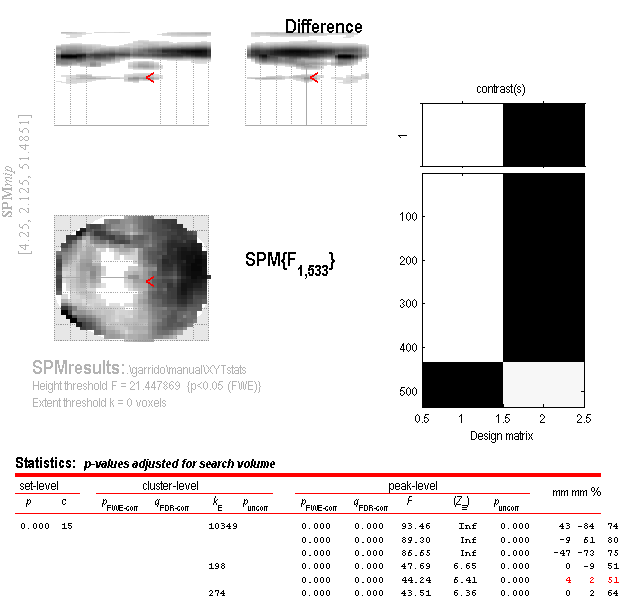
\includegraphics[width=120mm]{mmn/3DSPM}
\caption{\em In this SPM the time axis is reflected in the two MIP windows in the top row, with time proceeding from the bottom to the top of the page. The cursor has been positioned by selecting the third cluster in the results table. This occurs at time point 160ms post stimulus. The design matrix on the right hand side comprises two columns, the first for standard trials and the second for rare ones. \label{3DSPM}}
\end{center}
\end{figure}
Now:
\begin{itemize}
\item{Press the right mouse button in the MIP}
\item{Select ``display/hide channels''}
\item{Select the \texttt{maedffMspm8\_subject1.mat} file.}
\end{itemize}
This links the \texttt{SPM.mat} file with the M/EEG file from which the EEG images were created.
It is now possible to superimpose the channel labels onto the spatial SPM, and also to ``goto the nearest channel'' (using options provided after a right mouse click, when navigating the MIP).
 
We have demonstrated sensor space analysis for single-subject data. More frequently, one would compute ERP images for each subject, smooth them, and then perform paired t-tests over subjects to look for condition differences. See \cite{marta_mmndcm} for a group analysis of MMN data.
 
Finally, if one had more constrained a priori knowledge about where and when the differences would appear, one could perform a Small Volume Correction (SVC) based on, for example, a box around fronto-central channels and between 100 and 200ms poststimulus. We also refer the reader to chapter \ref{Chap:eeg:sensoranalysis} for further details on sensor space analysis.

\subsection{Batching statistics}
The abovedescribed steps can be automatised using the batch tool. The relevant modules can be found in the 'Stats' submenu of the 'SPM' menu. They are 'Factorial design specification', 'Model estimation', 'Contrast manager' and 'Results report'. We will not go over the batch steps in detail but you should be able to build the batch now based on previously described principles. One point worth mentioning is that preprocessing and statistics can be done in a single batch with dependencies. For that the 'Convert2Images' module can be added to the batch twice and the 'Conditions' option in this module can be used to convert the 'standard' and 'rare' conditions separately  in the two instances of the module to match the two separate dependencies from 'Factorial design specification'. 

\section{Source reconstruction}

Source reconstruction comprises forward modeling and inverse modeling steps and is implemented by pressing the 3D source reconstruction button in SPM's top-left window.
This brings up the source localisation GUI shown in Figure~\ref{source_gui}. The following subsections detail each of the steps in a source reconstruction analysis. We also advise the reader to consult the reference material in chapter \ref{Chap:eeg:imaging}.

\begin{figure}
\begin{center}
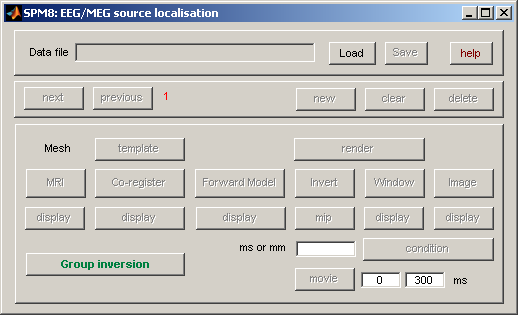
\includegraphics[width=120mm]{mmn/source_gui}
\caption{\em Graphical user interface for 3D source localisation. A complete localisation comprises the following steps (i) creation of a cortical mesh, (ii) co-registration of the mesh with M/EEG data, (iii) creation of a forward model, and (iv) results interrogation. As each of these steps is completed the relevant part of the GUI becomes highlighted (text appears more solid).
\label{source_gui}}
\end{center}
\end{figure}

\subsection{Mesh}
The first step is to load the data and create a cortical mesh upon which M/EEG data will be projected:
\begin{itemize}
\item{Press the ``Load'' button in the souce localisation GUI and select the file \texttt{maefdfMspmeeg\_subject1.mat}.}
\item{Enter ``Standard'' under ``Comment/Label for this analysis'' and press OK.}
\item{Now press the ``template'' button.}
\item{For ``Cortical mesh'', select ``normal''.}
\end{itemize}
SPM will then form the ``standard'' or ``canonical'' cortical mesh shown in the Graphics window which, after rotation, should look like Figure~\ref{mesh}
\begin{figure}
\begin{center}
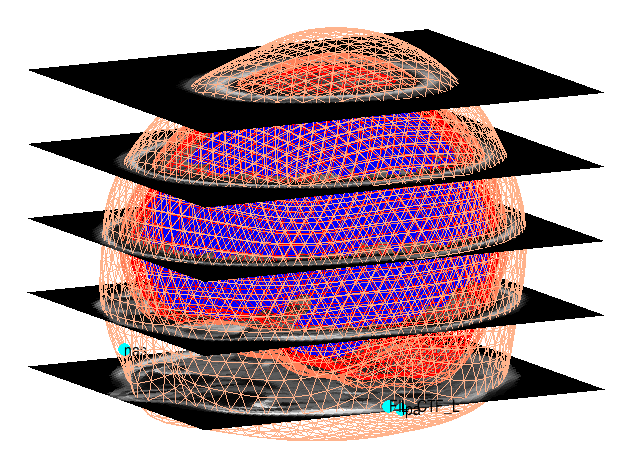
\includegraphics[width=120mm]{mmn/mesh}
\caption{\em The figure shows the canonical cortical mesh (blue), inner skull surface (red) and scalp surface (light brown). The hardwired fiducials are shown in light blue. Transverse slices of canonical MRI are also shown in black, with gray scale inlays showing anatomical detail.
\label{mesh}}
\end{center}
\end{figure}

\subsection{Coregister}

Now press the ``Co-register'' button. This will create further output in the Graphics window, the upper panel of which should like like Figure~\ref{coreg}.
\begin{figure}
\begin{center}
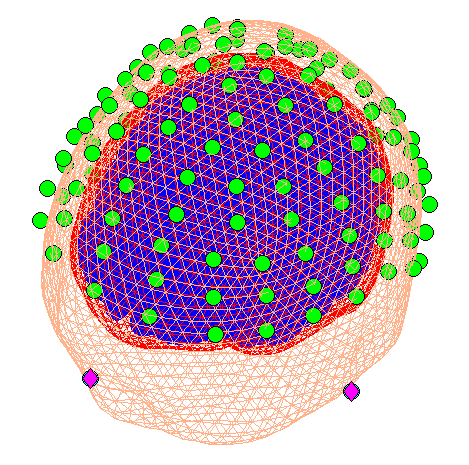
\includegraphics[width=120mm]{mmn/coreg}
\caption{\em
The figure shows the MRI fiducials (pink), the sensor fiducials (blue) and the locations of sensors (green) in addition the the canonical cortical mesh (blue), inner skull surface (red) and scalp surface (light brown).
\label{coreg}}
\end{center}
\end{figure}

In this coregister step we were not required to enter any further parameters. However, if you are not using the template (or ``canonical'' mesh) or if at the ``prepare'' stage above you loaded your own (non-standard) sensor positions then you will be asked for the locations in MNI coordinates of the fiducial positions.

\subsection{Forward model}

Now press the ``Forward model'' button. Then select ``EEG-BEM'' in response to the ``Which EEG head model?'' question. SPM will then use a Boundary Element Method (BEM) which will take approximately 10 minutes to run. Upon completion SPM will write the \texttt{single\_subj\_T1\_EEG\_BEM.mat} file into the canonical subdirectory of your SPM distribution. The Graphics window should now appear as in Figure~\ref{forward}.
\begin{figure}
\begin{center}
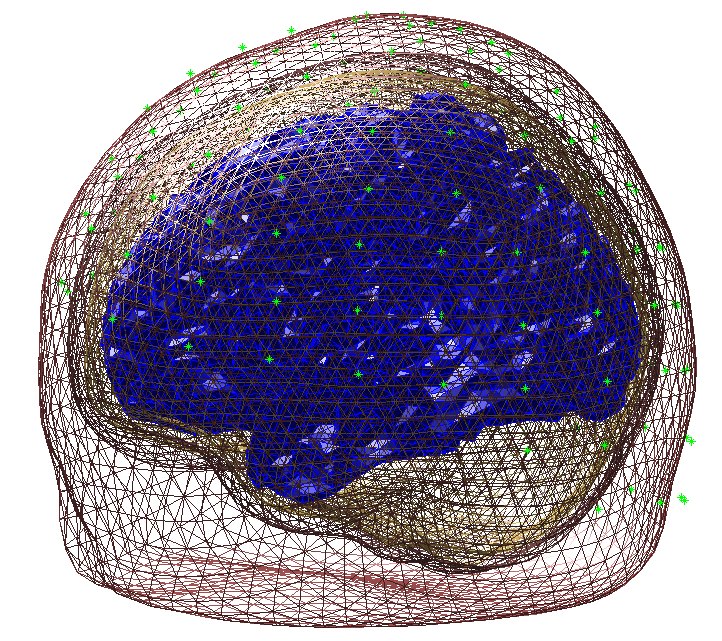
\includegraphics[width=120mm]{mmn/forward}
\caption{\em
The figure shows the cortical mesh (blue), brain, skull and scalp surfaces. Electrode positions are marked with asterisks.
\label{forward}}
\end{center}
\end{figure}
The next time you wish to use an EEG-BEM solution based on the template mesh, SPM will simply use the date from the \texttt{single\_subj\_T1\_EEG\_BEM.mat} file (so this step will be much quicker the next time you do it). The same principle applies to EEG-BEM solutions computed from meshes based on subjects individual MRIs.

\subsection{Invert}

Now press the Invert button and
\begin{itemize}
\item{Select an ``Imaging'' reconstruction.}
\item{Select ``Yes'' for ``All conditions or trials''.}
\item{Select ``Standard'' for Model.}
\end{itemize}
SPM will now compute a leadfield matrix and save it in the file \texttt{SPMgainmatrix\_maefdfMspmeeg\_subject1.mat} placed in \texttt{DATA\_DIR}. This file can be replaced with one computed using other methods for computing the lead field (e.g. methods external to SPM). The forward model will then be inverted using the Multiple Sparse Priors (MSP) algorithm (the progress of which is outputted to the \matlab\ command window). SPM will produce, in the Graphics window, (i) a Maximum Intensity Projection (MIP) of activity in source space (lower panel) and (ii) a time series of activity for (upper panel) each condition.

The ``ms or mm'' window has three functionalities (i) if you enter a single number this will be interpreted as ms, (ii) if you enter two numbers this will be interpreted as a time window for plotting movies (see below), (iii) if you enter 3 numbers this will be interpreted as MNI coordinates for a time series plot.

Now enter ``160'' for ``ms or mm'' and press the MIP button, to see a MIP of activity in source space at 160ms post-stimulus, and the time series of activities (top panel) at the position with largest magnitude signal. The corresponding graphic is shown in Figure~\ref{invert}. By toggling the ``Condition'' button, and pressing MIP each time, you can view the spatial distribution of activity for the different conditions (at the selected time point).
\begin{figure}
\begin{center}
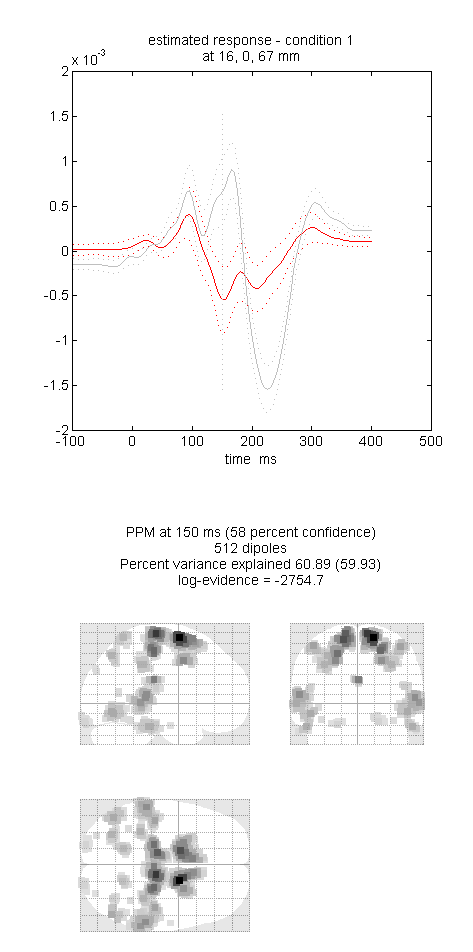
\includegraphics[width=120mm]{mmn/invert}
\caption{\em Source reconstructed activity at 160ms post-stimulus.
The upper trace shows responses to Condition 1 (Standards) with the red curve, and to Condition 2 (Rare) in gray.
\label{invert}}
\end{center}
\end{figure}

\subsection{Batching source reconstruction}
All the functionality of source reconstruction can be batched, using the tools from 'Source reconstruction' submenu of 'M/EEG'. 'Head model specification tool' performs mesh generation, coregistration and forward model specification. 'Source inversion' tool computes the inverse solution and 'Inversion results' tool summarises the inversion results as images. One tip when incorporating source reconstruction batch in a script is one should be aware that the batch reads the @meeg object from disk and saves the results to disk but does not update the @meeg object in the workspace. Thus, it is advised to save any changes to the object before running the batch (D.save) and to reload the object after running the batch (D = D.reload). 

\section{Dynamic Causal Modeling}

Many of the functionalities of DCM for M/EEG are described in more detail in the reference chapter \ref{Chap:eeg:DCM}. In this chapter we demonstrate only the ``DCM for ERP'' model. 
Users are strongly encouraged to read the accompanying theoretical papers \cite{od_dcm_erp,sjk_dcm_erp}. Briefly, DCM for ERP fits a  neural network model to M/EEG data, in which activity in source regions are described using differential equations based on neural mass models. Activity in each region comprises three populations of cells; pyramidal, local excitatory and local inhibitory. Fitting the model will then allow you to plot estimated activity in each cell population in each region. It will also provide estimates of the long range connections between regions, and show how these values are changed by experimental manipulation (eg. rare versus standard trial types).
  
In the \texttt{example\_scripts} folder of the SPM distribution, we also provide an example script that will run a DCM-for-ERP analysis of this data. This can be edited to implement your own analysis.

Pressing the ``DCM'' button will open up the DCM GUI shown in Figure~\ref{dcm_gui}.
\begin{figure}
\begin{center}
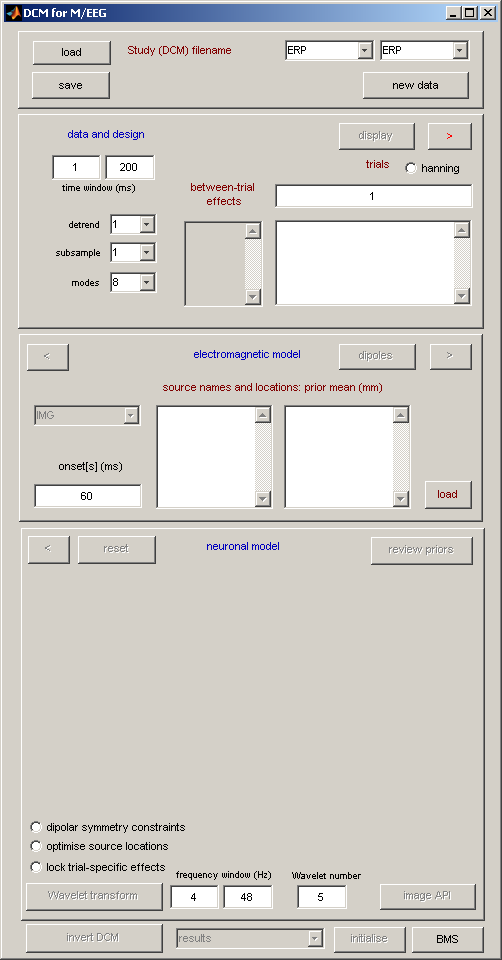
\includegraphics[width=80mm]{mmn/dcm_gui}
\caption{\em The Dynamic Causal Modeling GUI splits model specification into three reversible phases (i) data and design, (ii) electromagnetic model and (iii) neuronal model. One can move forwards and backwards in the model specification using the left and right arrow buttons (these become highlighted when sufficient information has been entered to proceed to the next step).
\label{dcm_gui}}
\end{center}
\end{figure}
\begin{figure}
\begin{center}
%\includegraphics[width=80mm]{mmn/}
(a)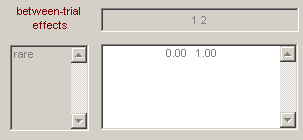
\includegraphics[width=80mm]{mmn/data_and_design}
(b)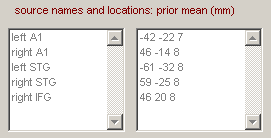
\includegraphics[width=80mm]{mmn/electro_model}
(c)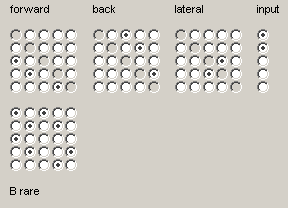
\includegraphics[width=80mm]{mmn/neuronal_model}
\caption{\em Specification of DCM for ERP model (a) Data and design, (b) electromagnetic model and (c) neuronal model.
\label{specify} }
\end{center}
\end{figure}
We will now complete the three model specification entries shown in Figure~\ref{specify}:
\begin{itemize}
\item{Press the ``new data'' button and select the \texttt{maedffMspm8\_subject1.mat} file.}
\item{Enter the ``between-trial effects'' and design matrix information shown in Figure~\ref{specify}(a).}
\item{Press the ``Display'' button.}
\end{itemize}
This completes the data specification stage. Now:
\begin{itemize}
\item{Press the right hand arrow to move on to the specification of the electromagnetic model.}
\item{Instead of ``IMG'' select ''ECD'' for the spatial characteristics of the sources.}
\item{Now enter the names and (prior mean) locations of the sources shown in Figure~\ref{specify}(b).}
\item{Pressing the ``dipoles'' button will create an interactive display in the graphics window showing the prior source positions.}
\end{itemize}
This completes the specification of the electromagnetic model. Now:
\begin{itemize}
\item{Press the right hand arrow (next to the dipoles button) to move on to specification of the neuronal model.}
\item{Highlight the connectivity matrix radio buttons so that they  correspond to those shown in Figure~\ref{specify}(c).}
\item{Press the (top left) 'save' button and accept the default file name.}
\item{Press 'Invert DCM'}
\end{itemize}
SPM will plot the progess of the model estimation in the MATLAB command window. Plots of data and the progressing model fit will be shown in SPM's graphics window. The algorithm should converge after five to ten minutes (in 64 iterations). Now select the ``ERPs (sources)'' option from the pull down menu to the right of the ``Estimated'' button. This will produce the plot shown in Figure~\ref{source_erps}. The values of the connections between areas can be outputted by selecting eg ''Coupling(A)'' from the pull-down menu in the DCM GUI. This will allow you to interrogate the posterior distribution of model parameters. It is also possible to fit multiple models, eg. with different numbers of regions and different structures, and to compare them using Bayesian Model Comparison. This is implemented by pressing the BMS button (bottom right hand corner of the DCM window).

\begin{figure}
\begin{center}
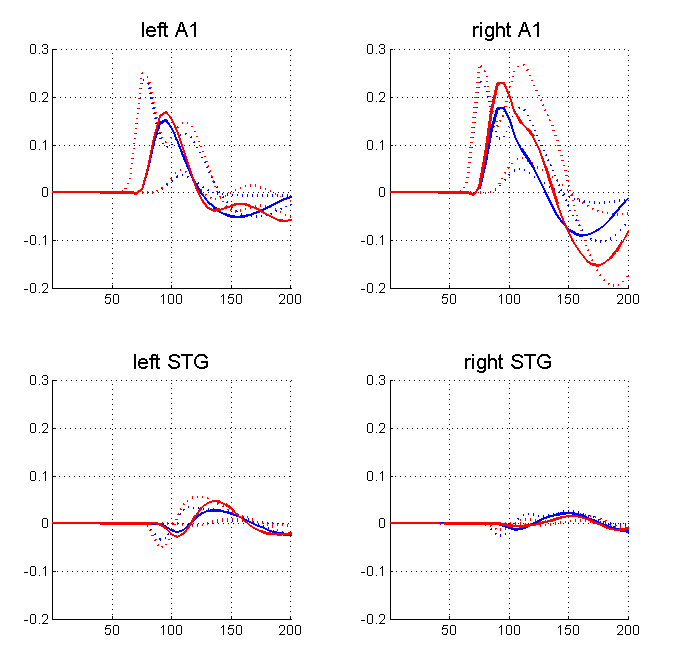
\includegraphics[width=120mm]{mmn/source_erps}
\caption{\em Activity plots for three neuronal populations (solid lines for pyramidal cells, dotted lines for others), in four areas (fifth not shown in this figure), for standard (blue) and rare (red) trial types.
\label{source_erps} }
\end{center}
\end{figure}
